\documentclass{beamer}
\usepackage{ctex, hyperref}
\usepackage[T1]{fontenc}

% other packages
\usepackage{latexsym,amsmath,xcolor,multicol,booktabs,calligra}
\usepackage{graphicx,pstricks,listings,stackengine}

\author{William Li}
\title{PHCS CS101}
\subtitle{Lecture1}
\institute{十二(8)}
\date{2023年10月10日}
\usepackage{Tsinghua}

% defs
\def\cmd#1{\texttt{\color{red}\footnotesize $\backslash$#1}}
\def\env#1{\texttt{\color{blue}\footnotesize #1}}
\definecolor{deepblue}{rgb}{0,0,0.5}
\definecolor{deepred}{rgb}{0.6,0,0}
\definecolor{deepgreen}{rgb}{0,0.5,0}
\definecolor{halfgray}{gray}{0.55}

\lstset{
    basicstyle=\ttfamily\small,
    keywordstyle=\bfseries\color{deepblue},
    emphstyle=\ttfamily\color{deepred},    % Custom highlighting style
    stringstyle=\color{deepgreen},
    numbers=left,
    numberstyle=\small\color{halfgray},
    rulesepcolor=\color{red!20!green!20!blue!20},
    frame=shadowbox,
}


\begin{document}

\kaishu
\begin{frame}
    \titlepage
    %\begin{figure}[htpb]
    %    \begin{center}
    %        
\includegraphics[width=0.2\linewidth]{pic/Tsinghua_University_Logo.eps}
    %    \end{center}
    %\end{figure}
\end{frame}

\begin{frame}
    \tableofcontents[sectionstyle=show,subsectionstyle=show/shaded/hide,subsubsectionstyle=show/shaded/hide]
\end{frame}


%\section{课题背景}

%\begin{frame}{用Beamer很高大上?}
    %\begin{itemize}[<+-| alert@+>] % 当然,除了alert,手动在里面插 \pause 也行
        %\item 大家都会\LaTeX{},好多学校都有自己的Beamer主题
        %\item 中文支持请选择 Xe\LaTeX{} 编译选项
        %\item Overleaf项目地址位于 \url{https://www.overleaf.com/latex/templates/thu-beamer-theme/vwnqmzndvwyb},可以直接使用
        %\item GitHub项目地址位于 \url{https://github.com/Trinkle23897/THU-Beamer-Theme},如果有bug或者feature request可以去里面提issue
%    \end{itemize}
%\end{frame}
\section{C++语言基础}
\subsection{C++语法}
\begin{frame}{Hello World}
    \begin{minipage}{0.45\linewidth}
        \begin{figure}
        \centering
        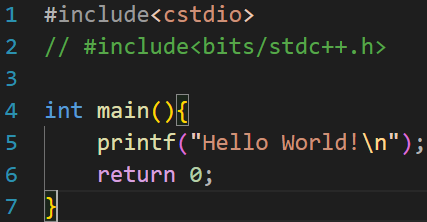
\includegraphics[width=\linewidth]{pic/Hello World.png}
        \caption{Hello World}
        \label{fig:helloworld}
    \end{figure}
    \end{minipage}
    \hspace{1cm}
    \begin{minipage}{0.37\linewidth}
        \begin{itemize}
            \item 头文件
            \item 主函数
            \item printf函数
            \item 返回值
        \end{itemize}
    \end{minipage}
\end{frame}
\begin{frame}{A+B Problem}
    \begin{minipage}{0.45\linewidth}
        \begin{figure}
        \centering
        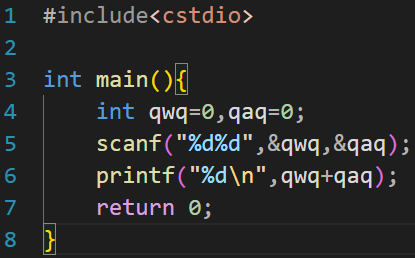
\includegraphics[width=\linewidth]{pic/A+B Problem.png}
        \caption{A+B Problem}
        \label{fig:A+BProblem}
    \end{figure}
    \end{minipage}
    \hspace{1cm}
    \begin{minipage}{0.37\linewidth}
        \begin{itemize}
            \item 定义变量
            \item scanf函数
            \item 运算符
        \end{itemize}
    \end{minipage}
\end{frame}
\begin{frame}{Variable Range}
    \begin{minipage}{0.45\linewidth}
        \begin{figure}
        \centering
        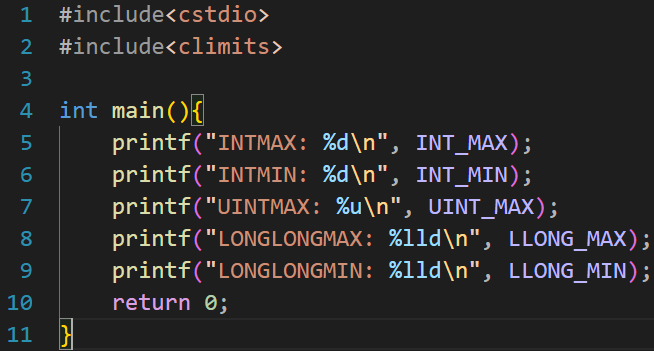
\includegraphics[width=\linewidth]{pic/Variable Range.png}
        \caption{Variable Range}
        \label{fig:variablerange}
    \end{figure}
    \end{minipage}
    \hspace{1cm}
    \begin{minipage}{0.37\linewidth}
        \begin{itemize}
            \item climits头文件
            \item 变量范围
        \end{itemize}
    \end{minipage}
\end{frame}
\end{document}